\documentclass[12pt,a4paper]{article}

% change to german
\usepackage[german]{babel}

% better hyphenation
\usepackage[final]{microtype}
\usepackage{csquotes}

% packages, images, math
\usepackage{geometry, graphicx, amsmath, amsfonts, array, multicol, multirow}

% for bibliography
\usepackage[
    backend=biber,
    style=alphabetic,
    sorting=ynt,
    minalphanames=3,
]{biblatex}
\addbibresource{./references.bib}


% colors
\usepackage[dvipsnames]{xcolor}

% for urls
\usepackage[colorlinks=true, urlcolor=blue, citecolor=blue, linkcolor=black]{hyperref}

% Remove Indentation at new line
\setlength{\parindent}{0cm}

% Set Font to Arial
% \usepackage{fontspec}
% \setmainfont{Arial}

% Set Font to Helvet
\usepackage{helvet}
\renewcommand{\familydefault}{\sfdefault}

% Set Layout
\geometry{
    a4paper,
    left=25mm,
    right=25mm,
    top=25mm,
    bottom=20mm
}

% Redefine title
\makeatletter
\def\@maketitle{%
  \newpage
  \null
  \vskip 2em%
  \begin{center}%
  \let \footnote \thanks
    {\Huge\bfseries\@title \par}%
    \vskip 1.5em%
    {\large
      \lineskip .5em%
      \begin{tabular}[t]{c}%
        \@author
      \end{tabular}\par}%
    \vskip 1em%
    {\large \@date}%
  \end{center}%
  \par
  \vskip 1.5em}
\makeatother

\begin{document}

\title{Supersonic Algorithms}
\author{Anton Rodenwald}

\maketitle

\large\begin{tabular}{l l}

    Projektbetreuerin: & Birgit Ziegenmeyer \\

    Institution: & Schillerschule Hannover \\
    
    Thema des Projektes: 
    & Analyse verschiedener Implementationen von Algorith- \\
    & men in Bezug auf die besten Techniken zur Optimierung \\
    & und Auseinandersetzung mit der Ausführung dieser, \\
    & um die Umsetzung hochperformanter und effizienter \\
    & Programme zu erforschen. \\

    Fachgebiet: & Mathematik/Informatik \\

    Wettbewerbssparte: & Jugend Forscht \\
    
    Bundesland: & Niedersachsen \\
    
    Wettbewerbsjahr: & 2023 \\
    
\end{tabular}


\clearpage
\section*{Kurzfassung}
Nachdem wir im Informatikunterricht der SEK II Sortieralgorithmen behandelt hatten,
stellte ich mir die Frage, wie man am schnellsten eine Liste von 10 Millionen zufällig Generierten Zahlen
sortieren kann und welche Programmiersprache und welche Techniken man nutzen sollte.
Daraus entwickelte sich dann die etwas allgemeinere Fragestellung, 
nämlich welche Optimierungen erhöhen die Ausführgeschwindigkeit von Programmen am meisten und wieso?
Mir war bekannt, dass Python, was wir im Unterricht verwendet hatten, als eine der langsamsten Sprachen gilt, 
weswegen ich neben Python auch noch C++ wählte, was allgemein als eine der schnellsten Sprachen gilt.
Ich implementierte anschließend verschiedene Variationen der Quicksort und anderer Algorithmen und testete so, 
in welchem Maß Optimierungsansätze die Performance beeinflussten.
Dabei kam ich zu dem Ergebnis, dass die besten Python Bibliotheken zur Optimierung "numpy" und "numba" waren,
wobei C++ trotzdem schneller war, womit sich meine Hypothese bestätigte.
Dies erklärte ich mir dadurch, dass Python eine Interpretierte und C++ eine kompilierte Sprache ist, diese
beiden Sprachen also gänzlich verschiedenen sind und somit auch die Möglichkeiten zur Optimierung dieser Andere sind.
Schlussendlich gelang es mir noch unter Nutzung von AVX2, einem speziellen Befehlssatz, in C++ eine 4x schnellere Version als die standardmäßig 
Vorhande zu entwickeln was mir zeigte, dass es im Gebiet der Codeoptimierung noch viel zu entdecken und zu
testen gibt.
Im breiteren Kontext gesehen, sind Optimierungen hilfreich, um die Ausführung von Programmen aller Art zu Optimierungen,
was zur Einsparungen von monetären und natürlichen Ressourcen führen kann und konkret bei Unternehmen den Gewinn
vervielfachen kann.

\clearpage
\renewcommand*\contentsname{Inhaltsverzeichnis}
\tableofcontents

\clearpage

\section{Einleitung}

Im Informatik Leistungskurs des 12. Jahrgangs beschäftigten wir uns nach den Herbstferien mit
der Laufzeit von Algorithmen am Beispiel der Quicksort, einem Sortieralgorithmus.
Nach diesem thematischen Impuls ergab sich mein Projekt zur Erforschung von Sortieralgorithmen,
in dem ich es mir zuerst zur Aufgabe gemacht hatte, den schnellsten Weg zu finden, 10 Millionen zufällig
generierte Zahlen zu sortieren. Mein Fokus änderte sich dann allerdings und ich fokussierte mich
auf die Aspekte der Implementation und tatsächlichen Ausführung der Programme, da 
Sortieralgorithmen algorithmisch bereits sehr weit erforscht sind und man in diesem Gebiet nur
sehr schwer neue Erkenntnisse sammeln konnte \cite{sortieralgorithmenwikipedia}.
Ich entschied mich deswegen, nicht nach besseren Algorithmen zu suchen, sondern nach Wegen, 
mein ursprüngliches Program in Python in seiner Ausführung zu beschleunigen und so vorteilhafte
Wege der Geschwindigkeitsoptimierung zu entdecken.
Ich stellte mir die Frage, welche Optimierungen die Ausführgeschwindigkeit von Programmen
am meisten erhöhen und wieso?
Zum Thema der Optimierung fand ich im Bezug auf Python einige Bibliotheken im Internet, die
bessere Performance versprachen, von denen ich einige auswählte, um herauszufinden,
welche dieser den größten Geschwindigkeitsboost bringt.
Außerdem entschied ich mich noch dazu, einige Algorithmen auch in C++ zu implementieren, wobei ich im Bezug 
darauf nicht direkt Möglichkeiten und Erklärungen fand, welche Modifikationen ein Program schneller machen und
wieso diese Veränderungen es schneller machen.
Weiterführend verglich ich noch, wie sich meine C++ Programme mit denen in Python in der Ausführung auf einer
tiefergreifenden Stufe unterschieden, um herauszufinden, wieso C++ meist deutlich schneller ist.
Meine Erwartung war dabei, dass C++ bei jeder Aufgabe Python um ein vielfaches übertrifft im Punkt der Geschwindigkeit,
da Python im allgemeinen als langsam gilt und C++ als sehr performant und schnell.

\clearpage

\section{Vorgehensweise, Materialien, Methode}

\subsection{Vorgehen}
Meine Vorgehensweise beruhte darauf, mich im Internet über Möglichkeiten der Optimierung zu informieren und diese geschickt neu zu kombinieren und die erreichten Geschwindigkeiten miteinander zu vergleichen, wodurch
ich eine Qualitative Entscheidung treffen konnte, welche Variationen die größten Performanceverbesserungen bringen.
Dazu wählte ich die Python Bibliotheken \textit{numpy}, \textit{numba}, \textit{ctypes} und \textit{cython} und
testete auch Funktionen aus den Standardbibliotheken der Sprachen.
Bei der Implementation nutzte ich Internetquellen wie Stackoverflow, die Cython Dokumentation und andere 
(alle Seiten aufzuzählen ist nicht zielfführend), um die Implementierung umzusetzen, 
da ich noch kaum Erfahrung mit diesen Bibliotheken hatte \cite{stackoverflow} \cite{cythondocs}.
Dies wurde besonders wichtig beim implementieren in den mir noch kaum bekannten Sprachen Java, Lua, Julia und Go.
Meine Implementationstechnik war das iterative Implementieren, wo ich eine Startversion immer wieder abwandelte und
konstant Dinge änderte. Dabei behielt ich immer die Ausführungszeit im Auge und entschied so, welche Ansätze
weitere Tests erforderten.
Bei der Implementation einer Radixsort, einem sehr schnellen Sortierverfahren, nutze ich außerdem 2 Publikationen 
zur Verbesserung meiner eigenen Variante und schuf so die Untergrenze all meiner getesteten Implementationen
\cite{terdiman} \cite{michael}.
Im Zuge dessen beschäftigte ich mich auch mit dem Konzept von AVX2 und nutze diesen erweiterten Befehlssatz, den
ich im Rahmen der Ergebnisse noch weiter beschreiben werde.
\cite{intelavxdocs} \cite{avxguide}.



\clearpage

\subsection{Materialien}
Für mein Projekt nutze ich meinen Desktop PC (Linux) und meinen Laptop (Linux) zur Implementation und Ausführung der Programme.
Dabei nutze ich verschiedene Arten von Software zum entwickeln und Ausführen meiner Programme und zum erstellen meiner
schriftlichen Arbeit. \newline

Ich nutze dabei diese Software in der jeweiligen Version:
\begin{itemize}
    \item Visual Studio Code (Editor für Code)
    \item \LaTeX (Erstellen der Dokumentation)
    \item clang++ 14.0.6 (C/C++ Compiler)
    \item python 3.10.8 (Ausführen der Dateien)
    \item java 19.0.1 openjdk (Javac, JVM)
    \item lua 5.4.4 (Ausführen der Dateien)
    \item nodejs 18.8.0 (Ausführen der Dateien)
    \item julia 1.8.3 (Ausführen der Dateien)
    \item go 1.19.4 (Compilierung)
\end{itemize}


\subsection{Methode}

Meine Methode war das strukturierte Testen und vergleichen von Programmimplementationen und ihrer 
Variationen mithilfe einer einfachen Zeitname. Ich nutze die Möglichkeiten der jeweiligen Programmiersprachen, 
um die Ausführungszeiten auf die Milisekunde genau oder sogar genauer zu bestimmen und 
so zu vergleichen zu machen. In Python definierte ich mir dafür eine eigene Klasse (Abb. 1), fügte das Starten und Stoppen
des Timers meinem code hinzu (Abb. 2) und ließ mir die Ergebnisse als Text ausgeben (Abb. 3).
Damit die Ergebnisse vergleichbar sind, implementierte ich immer auf ähnliche Weise die Algorithmen und
nutze die gleichen Eingabewerte und Konstanten.
Als Beispiel generierte ich mir in jeder Sprache eine Liste aus 10 Millionen Zufallszahlen,
was ich nicht in die Zeit mit einbezog, und wendete auf diese dann die implementierten Algorithmen an.
So hatten alle Programme die Gleiche Aufgabe zu lösen, wodurch Vergleichbarkeit gewährleistet ist.
Wichtig war auch, die finalen Tests direkt nach einem Neustart des PCs ohne andere laufende Programme
zu machen, damit es durch variierende Prozessorauslastung keine Verfälschungen gab. 

\begin{multicols}{2}
    
    \begin{center}
        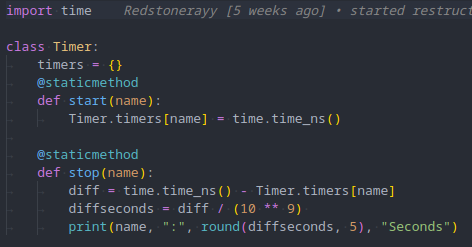
\includegraphics[width=.5\textwidth]{screenshots/pythontimer.png}
        Abb. 1
    \end{center}
    
    \columnbreak
    
    \begin{center}
        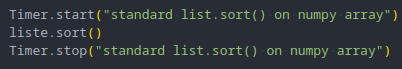
\includegraphics[width=.5\textwidth]{screenshots/timerexample.png}
        Abb. 2
        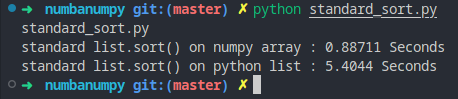
\includegraphics[width=.5\textwidth]{screenshots/outputexample.png}
        Abb. 3
    \end{center}
    
\end{multicols}

\subsection{Schwierigkeiten}
Die größte Schwierigkeit war, dass ich auf diesem Themengebiet noch nicht sehr viel Vorerfahrung hatte.
Außerdem waren die Konzepte teils komplex und es war nicht immer einfach, im Internet gute Beispiele zur Implementierung
zu finden. Vor dem Projekt hatte ich mich z. B. noch nie mit der Python Bibliothek "ctypes" beschäftigt und deshalb fand
ich meist erst nach längerem Suchen im Internet eine Lösung für auftretende Fehler.
Auch bei der Implementation von Programmen in C++ hatte ich teils meine Schwierigkeiten, da das Verstehen
von einigen Bitoperationen erstmal ein eindenken in die Thematik erforderte.
Mit dem Ausführen der Programme hatte ich hingegen kaum Probleme.
Ein für mich nicht lösbares Problem war auch die Implementierung in Go, wo nur dass generieren
einer 7 Millionen Zahlen langen Liste möglich, da bei mehr Zahlen mehr Arbeitsspeicher benötigt wurde,
als Go in einem Programmteil erlaubt. Der hohe Verbrauch an Arbeitsspeicher kommt meinen Vermutunge
nach von der Implementation von Recursion in Go, die nicht für sehr Tiefe Rekursion geeignet scheint
\cite{godeeprecursions} \cite{goroutinesize}.



\clearpage
\section{Ergebnisse}

\begin{center}
    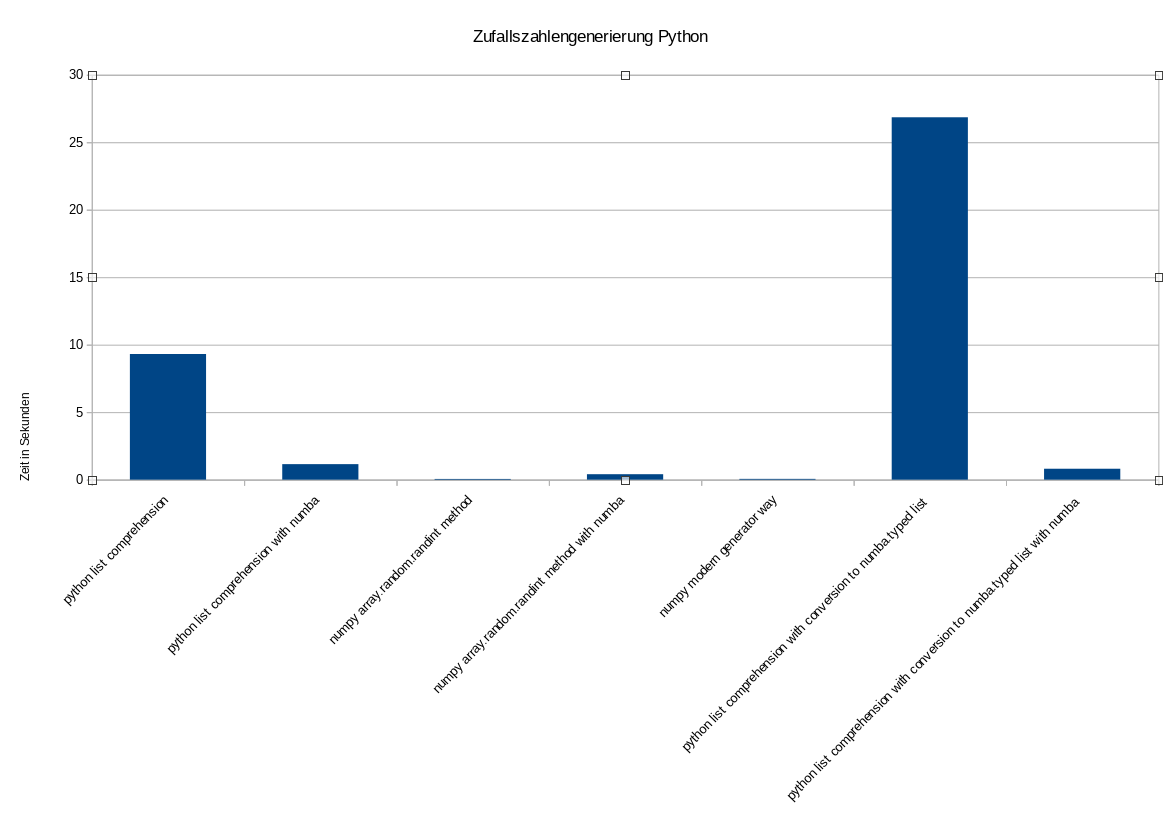
\includegraphics[width=1\textwidth]{./diagramme/bilder/listengenerierung.png}
\end{center}

\begin{center}
    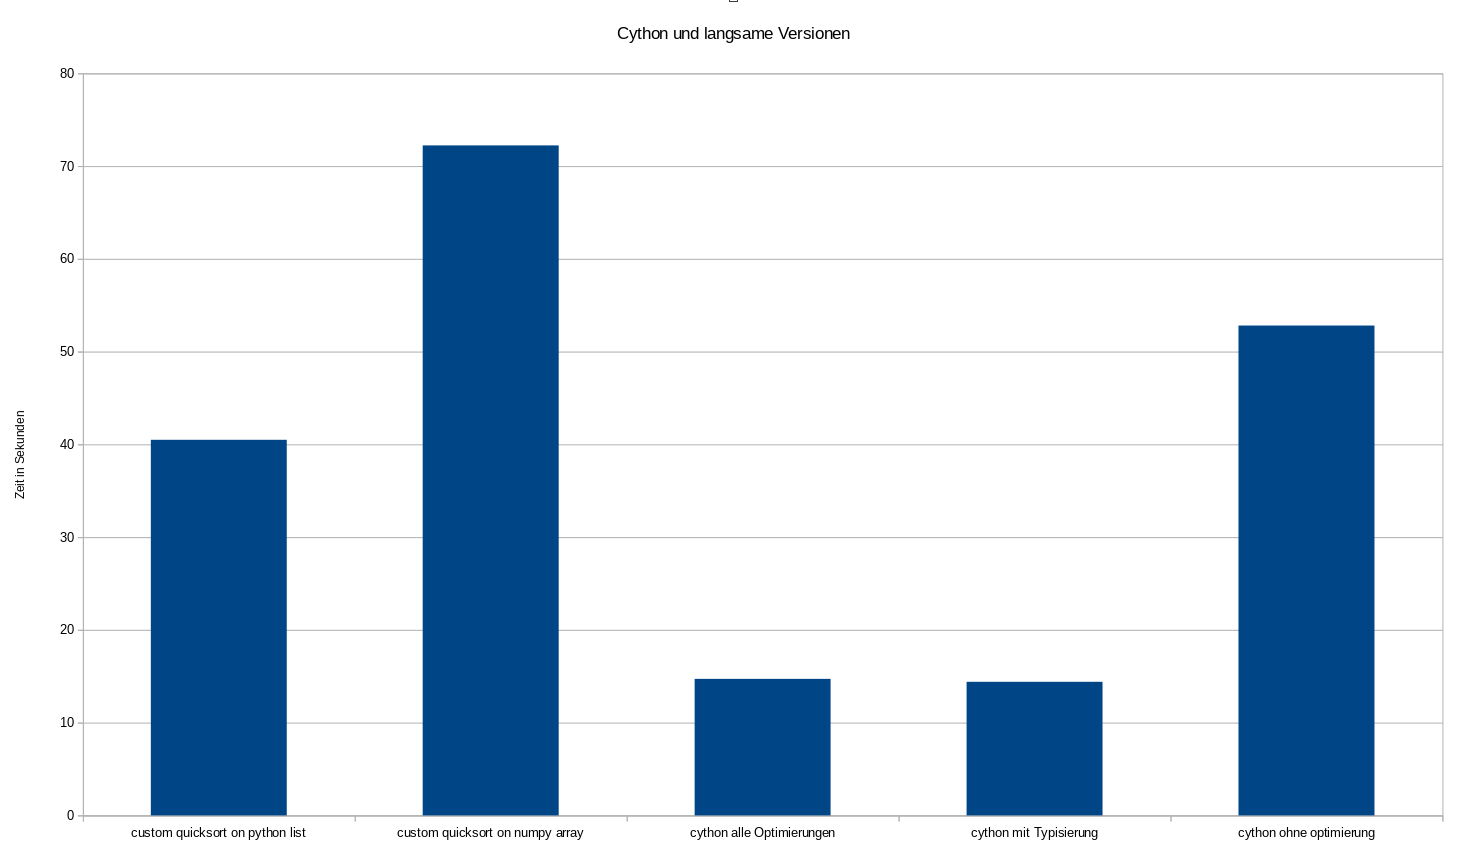
\includegraphics[width=1\textwidth]{./diagramme/bilder/sortierungen_cython_langsam.png}
\end{center}

\begin{center}
    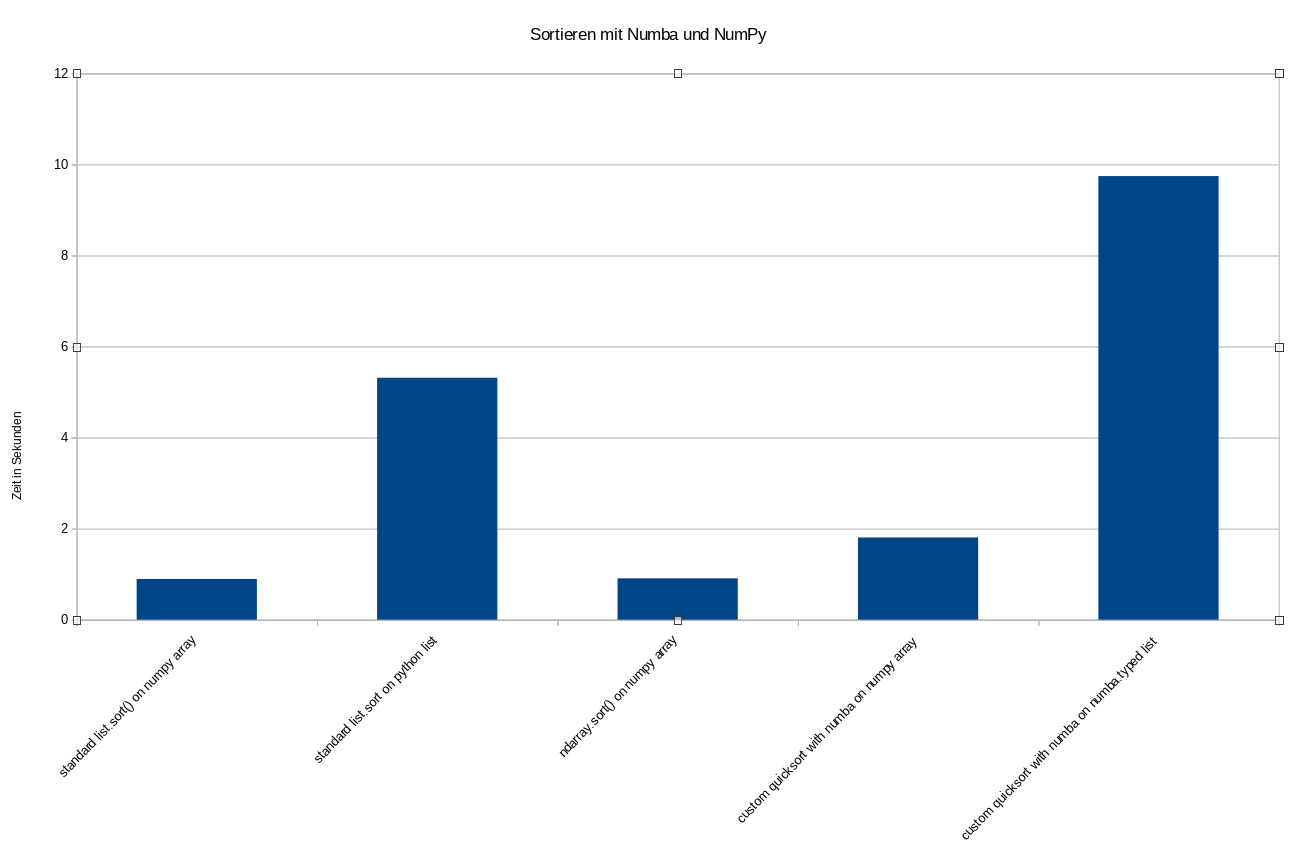
\includegraphics[width=1\textwidth]{./diagramme/bilder/sortieren_numba_numpy.png}
\end{center}

\begin{center}
    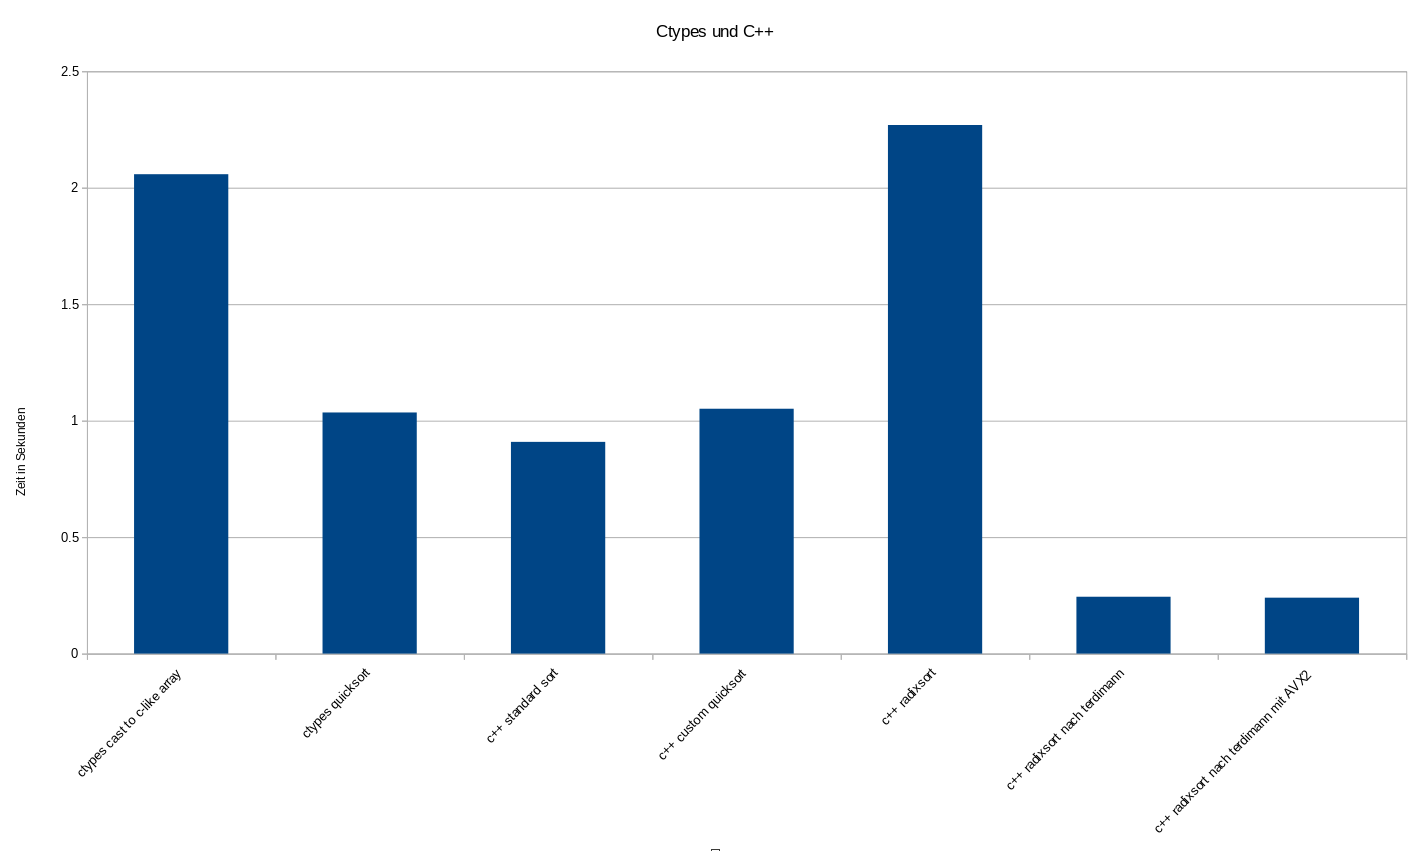
\includegraphics[width=1\textwidth]{./diagramme/bilder/ctypescpp.png}
\end{center}

\begin{center}
    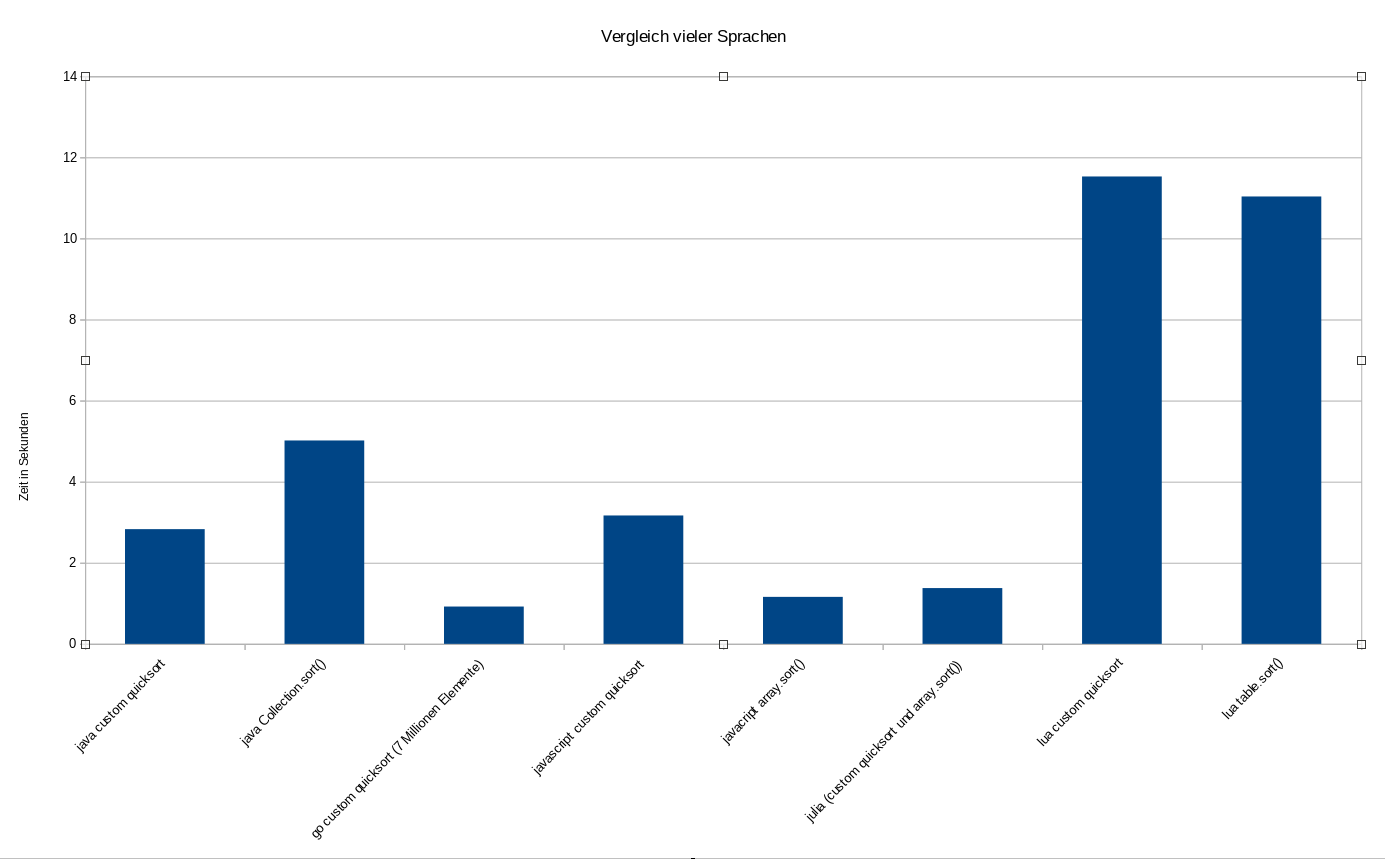
\includegraphics[width=1\textwidth]{./diagramme/bilder/comparison.png}
\end{center}

Zufallszahlengenerierung

Langsam

NumPy numba

c++, ctypes

Vergleich der Sprachen

\clearpage
\section{Diskussion}
\clearpage
\section{Zusammenfassung}

\clearpage

\printbibliography[title={Literaturverzeichnis}]

\end{document}